\documentclass[journal,10pt]{IEEEtran}
\IEEEoverridecommandlockouts
% The preceding line is only needed to identify funding in the first footnote. If that is unneeded, please comment it out.
\usepackage{cite}
\usepackage{amsmath,amssymb,amsfonts}
\usepackage{textcomp}
\usepackage{xcolor}
\usepackage{mathrsfs}
\usepackage{bbm}
\usepackage{indentfirst}
\usepackage{color}
\usepackage{cases}%���������{amsmath}����
\newcounter{mytempeqncnt}
\usepackage{booktabs}
\usepackage{graphicx}
\usepackage{multirow}
\usepackage{diagbox}
\usepackage{subfigure}
\usepackage{caption}
\usepackage{makecell}
\usepackage{threeparttable}
\usepackage{algorithm}
\usepackage{algorithmic}
\usepackage{setspace}
%\doublespacing
\usepackage{dsfont}
\usepackage{epstopdf}
\usepackage{bm}
\newtheorem{theorem}{Theorem}
\newtheorem{proof}{Proof}
\def\BibTeX{{\rm B\kern-.05em{\sc i\kern-.025em b}\kern-.08em
    T\kern-.1667em\lower.7ex\hbox{E}\kern-.125emX}}
\begin{document}

%\title{Stackelberg-Game-based Uplink Power Control in D2D-Enabled Vehicular Communication Networks}
\title{Robust Game-based Interference Management for Air-Ground Integrated Communications in Heterogeneous Vehicular Networks}
%Robust Game-Based Resource Allocation for UAV-assisted Ultra-dense Vehicular Networks
%Robust Game-based Resource Allocation for Air-Ground Integrated Communications in Ultra-Dense Vehicular Networks
%Robust Game-based Resource Allocation for Air-Ground Integrated Ultra-Dense Vehicular Networks
\author{Zhixin Liu,~\IEEEmembership{Member,~IEEE}, Jiawei Su, Yuan'ai Xie, Yazhou Yuan, Yi Yang and Xinping Guan, ~\IEEEmembership{Fellow,~IEEE}

\thanks{Zhixin Liu, Jiawei Su, Yuan'ai Xie, Yazhou Yuan and Yi Yang
are with the School of Electrical Engineering, Yanshan
University, Qinhuangdao 066004, China. Emails: lzxauto@ysu.edu.cn, Sjw@stumail.ysu.edu.cn,
 xieyuan\_ai@163.com, yzyuan@ysu.edu.cn, yyi@ysu.edu.cn}
\thanks{Xinping Guan is with School of Electronic, Information and Electrical Engineering, Shanghai Jiaotong University, Shanghai 200240, China. Email: xpguan@sjtu.edu.cn.}}

\markboth{Manuscript}
{}
%{Shell \MakeLowercase{\textit{et al.}}: Bare Demo of IEEEtran.cls for Journals}
\maketitle

\begin{abstract}
With the deployment of vehicular networks, air-ground integration is a potential scheme for interference-restricted terrestrial communications. This paper studies how to apply game theory to realize a well-function air-ground integrated heterogeneous vehicular networks (AGHVN), where the uplink channel allocated to the cellular user (CUE) is reused by multiple vehicle users (VUEs). In the heterogeneous vehicular communication scenarios with dense users, multi-user interference always leads to extremely poor communication quality. Moreover, the wireless channel is always time-variant, which further affects the system stability. To achieve effective and stable communications, game-based resource allocation scheme is placed great expectations in this paper. Considering a non-cooperative setting where the CUE and VUEs are selfish and profit-driven, a robust Stackelberg game framework is adopted to model the hierarchical competition, where the CUE and VUEs act as the leader and followers, respectively. Unlike traditional game schemes, the system robustness is highlighted by handling the channel uncertainty which is embedded in the interference constraints. Furthermore, a distributed algorithm is presented to obtain the game equilibrium (GE) solutions. Numerical results indicate that the proposed algorithm is effective and outperforms the benchmarks in robustness.
\end{abstract}

\begin{IEEEkeywords}
Vehicular networks, robust game, air-ground integrated communications, power control, channel uncertainty.
\end{IEEEkeywords}

\section{Introduction}

As the most promising solution for Intelligent Transportation Systems (ITS), Internet of Vehicles (IoV) is expected to meet rapidly growing demands, such as traffic efficiency,  driving experience, and accident handling \cite{TFL}. However, due to the rapid increase of vehicle density and user demand, single-cell network has a low spectrum efficiency. Therefore, the deployment of heterogenous vehicular networks has become a tendency.

Recently, as one of the most feasible solution to enhance the wireless communication quality, air-ground integration has attracted extensive attention from industry and academia. Due to the flexible deployment, remote operation, and relay capability, unmanned aerial vehicles (UAVs) in the air are selected to assist the terrestrial network \cite{ACO}. However, when UAVs join in the heterogenous scenarios, the air-ground integrated communication networks will face two major challenges. Firstly, multi-user interference is a tricky problem when channel reusing mode is used to improve spectrum efficiency. Effective and robust communications are greatly affected by the multi-user interference, especially in the uncertain channel environment, so it is a significant challenge to realize effective interference management \cite{ASO}. Secondly, the air-ground integrated heterogeneous vehicular networks (AGHVN) is hierarchical where the cellular user (CUE) and vehicle users (VUEs) act as the leader and the followers, respectively. However, the CUE and VUEs are different stakeholders who compete for their benefits. It is challenging to balance the interests of all parties. Hence, the widespread deployment of the air-ground integrated heterogeneous vehicular networks still poses urgent challenges.

Extensive attention and researches have been devoted to the area of air-ground integrated communications \cite{OUC}-\cite{SDR}. The authors focus on the air-ground integrated network architecture design and resource management \cite{OUC}, \cite{OSI}. In the heterogeneous cellular networks, the UAV is utilized to assist with emergency communications \cite{DUE}. A control framework that dynamically slices the spectrum resource for vehicular users is proposed in \cite{SDR}, where Lyapunov optimization theory is adopted. However, despite the above works have paid attention to improve performance in AGHVN, the research on combining system robustness and resource allocation has not received enough attention. Due to the existence of channel uncertainty, the existing resource allocation strategies are tricky to achieve the robust communications. Therefore, it is necessary to consider the impact of uncertain factors caused by movement, occlusion, noise and other factors on the robust transmission in AGHVN.

To overcome the above challenges, we propose a robust Stackelberg game-based resource allocation framework. Different from the conventional hierarchical game \cite{HUP}, \cite{DPC}, the proposed Stackelberg game includes robust power control scheme and price mechanism in this paper. The robust power control scheme introduces probability constraint to realize interference management. Furthermore, exponential integral method is adopted to transform the uncertain form into a solvable closed expression. Especially, price mechanism is adopted to combine with power control scheme. In the price mechanism, interference is regarded as a resource that can be allocated to VUEs. By charging for interference, CUE can improve its utility. However, when a VUE wants to obtain a higher rate by increasing transmission power, it has to pay more interference fees. Therefore, price mechanism can limit the selfish behavior of VUEs, thereby balancing the interests of all parties.


%The Internet of Vehicles (IoV) is expected to meet rapidly growing demands, such as traffic efficiency, road safety, driving experience, and accident handling. To ensure that the vehicles can get satisfactory services anytime and anywhere, an extremely versatile network is required to guarantee stable and efficient information transmission. To this end, an air-ground integrated vehicular networks (AGVN) is proposed as a promising networking structure, where unmanned aerial vehicles (UAV) are used to complement terrestrial communications \cite{ACO}, \cite{OUC}. With the characteristics of size miniaturization, remote operation, fast response, and controllable agility, UAV is deemed as a feasible solution to enhance the wireless communication quality.

%Although trajectory design is an important field of UAV research, in ultra-dense vehicle communication scenarios, the transmission benefit obtained by trajectory planning is not obvious. At the same time, fixed hovering and full coverage of multiple UAVs can greatly reduce the energy consumption \cite{EMC}.

\subsection{Contributions}
In this paper, a robust Stackelberg game-based resource allocation algorithm is proposed. The main contributions are summarized as follows:
\begin{itemize}
    \item The multi-user joint communication scenario in the the air-ground integrated heterogeneous vehicular networks is focused on, and effective interference management which is embedded in the probability constraints is highlighted to ensure the system robustness and the communication qualities.
    \item More practical vehicular communication environments with channel uncertainty are considered, a robust Stackelberg game framework is proposed to realize system stability. Especially, the proposed price mechanism works well to limit selfish behavior and balance the utilities of vehicle users.
\end{itemize}


\section{Problem Formulation}
\subsection{System and Channel Models}
We consider an uplink air-ground integrated communication scenario where numerous  vehicle-to-UAV (V2U) cells underlay a macrocell. As depicted in Fig. 1, UAVs are fixed hovering and deployed to the traffic-congested sections, they are responsible for receiving signals from vehicles within its coverage and transmitting them to the base station (BS). It is relevant to point out that all UAVs are duplex equipped with a receiving antenna and a transmitting antenna, so the process of receiving and transmitting can be finished at the same time. The sets of CUE and VUEs on communication are indexed as $\mathcal{S}_0:= \{0\}$ and $\mathcal{S}_l:=\{1, 2,..., N\}$, respectively. To improve the spectrum utilization and realize multi-user joint communication, V2U communications reuse the CUE's uplink channel. However, serious multi-user interference is produced which limits the communications of signal links. As shown in Fig. 1, signal link (cellular link and cochannel V2U link) and interference link (CUE-V link, V-BS link, and V2U interference link) are distinguished.
%The set of all users is then denoted as $\mathcal{S} := \mathcal{S}_0 \cup \mathcal{S}_l$. fixed hovering and full coverage of multiple UAVs can greatly reduce the energy consumption \cite{EMC}.
%In the $n${th} V2U cell, VUEs establish communication links with UAV$_{n}$ by reusing the CUE's uplink channel, $n\in\mathcal{S}_l$. To avoid inter-cell interference, the time division multiple access (TDMA) communication technology is adopted. Time resource is divided into multi-frames, and each frame is divided into several time slots. Different VUEs access its time slots when they communicate with the UAV, and signal transmission in different time slots will produce no interference \cite{TMF}. Hence, the intra-cell interference can be ignored in a time slot.



%As the most tricky feature of the ultra-dense scenarios, serious multi-user interference is also shown in Fig. 1.



Assuming that UAVs have the flight height $H_n$, the distance between VUE$_{k}$ and UAV$_{n}$ is
\begin{eqnarray}\label{1}
h_{k,n}=\sqrt{H_n^2+(\|W_k-W_n\|)^2},           &k\in \mathcal{N}, n\in \mathcal{N}
\end{eqnarray}
where $W_k$ and $W_n$ are the positions of VUE$_{k}$ and UAV$_{n}$. The distance between CUE and the BS is
\begin{eqnarray}\label{2}
h_{0,0}=\sqrt{H_0^2+(\|W_0-W_{BS}\|)^2},
\end{eqnarray}
where $W_0$ and $W_{BS}$ are the positions of CUE and BS, $H_0$ is the vertical height of the signal receiver on the BS. The distance between VUE$_{k}$ and the BS is $h_{k,0}$, the distance between CUE and UAV$_{n}$ is $h_{0,n}$. The expressions of $h_{k,0}$ and $h_{0,n}$ are similar to (\ref{1}) and (\ref{2}).

\begin{figure}[htbp]
\centerline{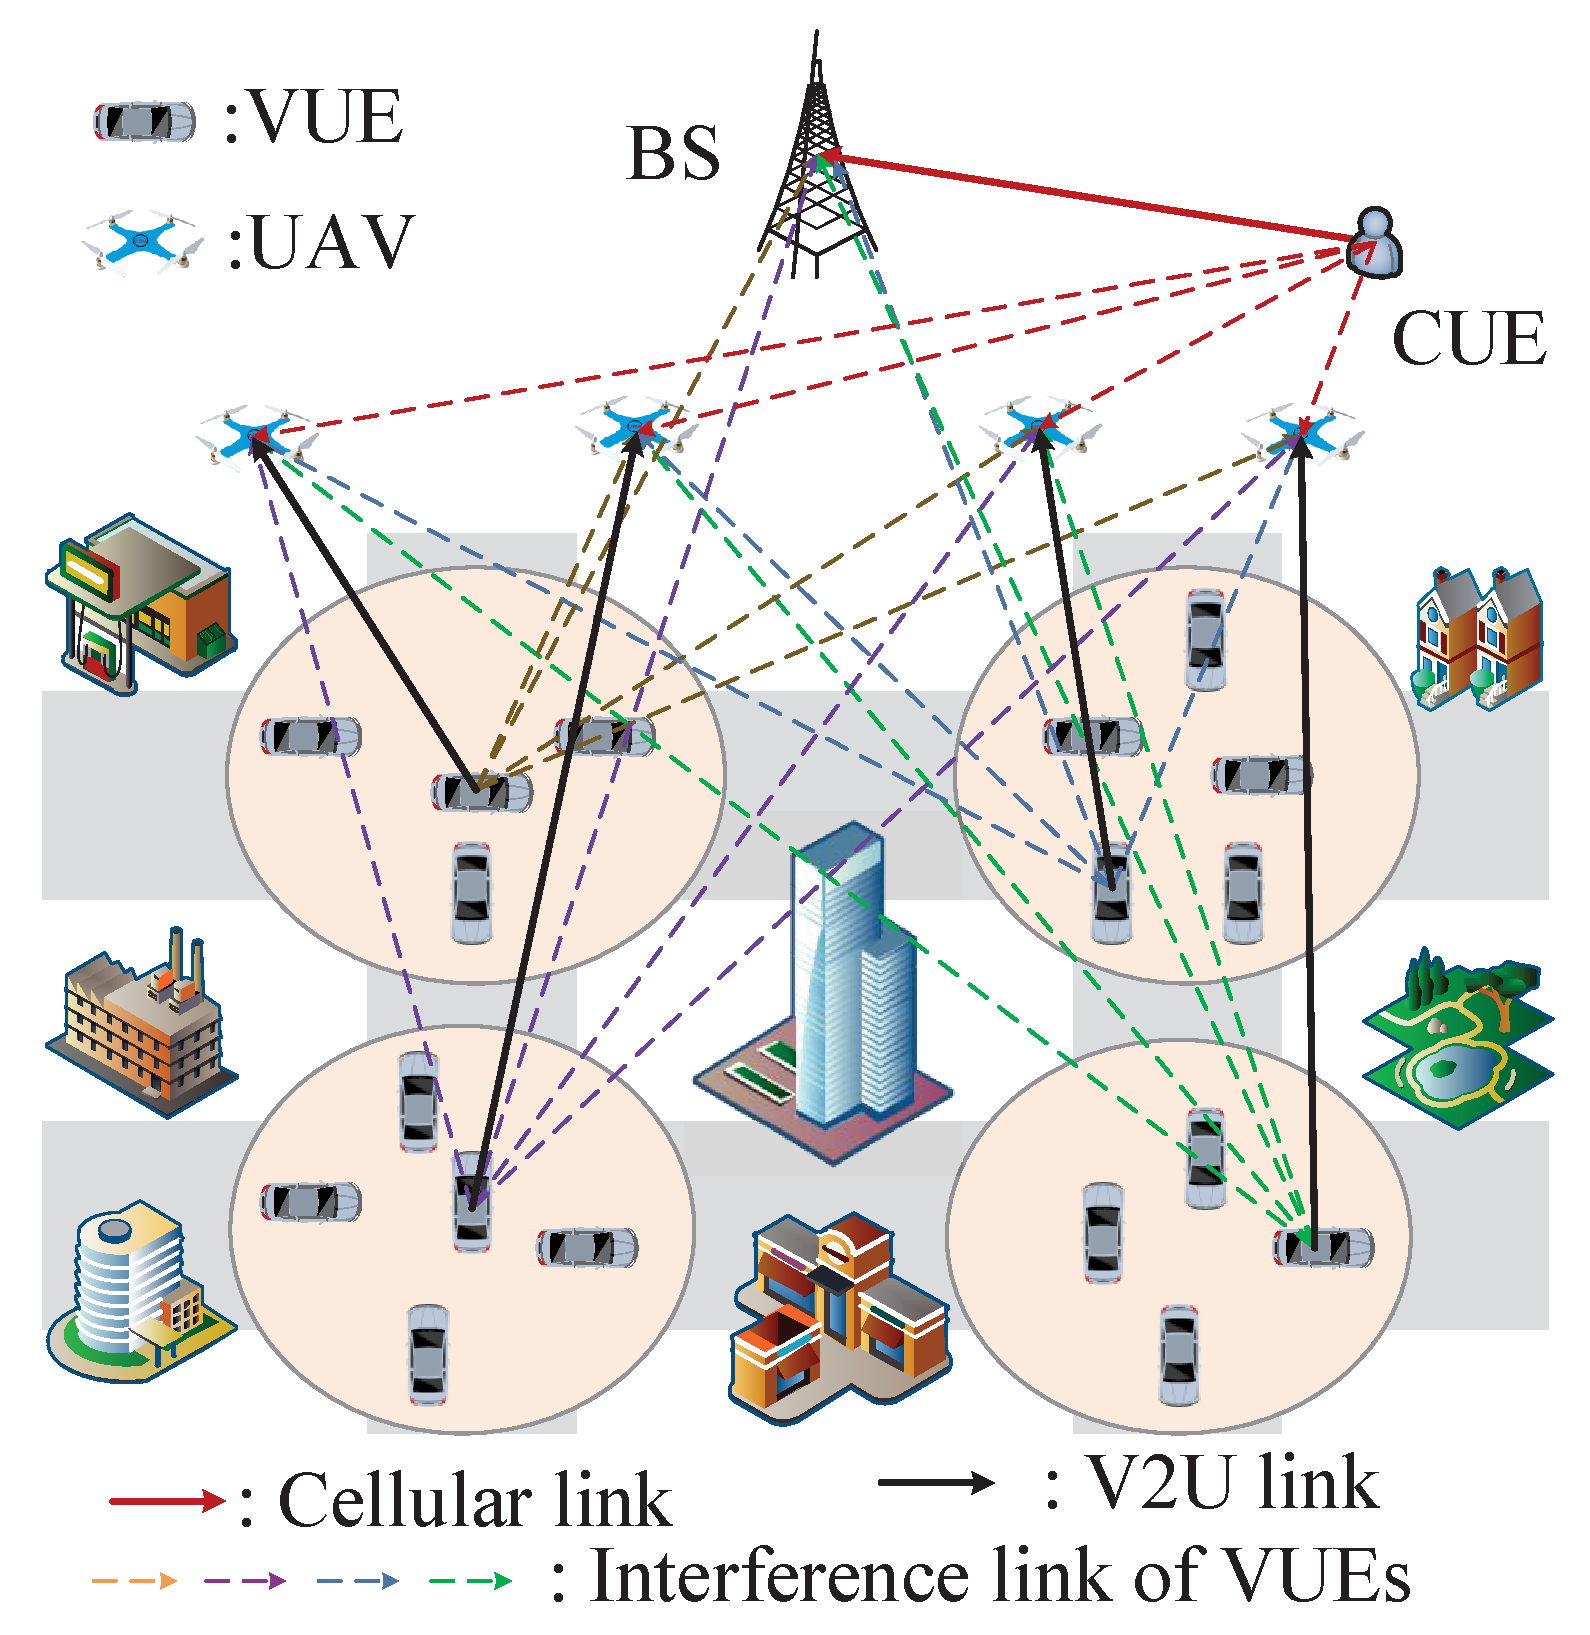
\includegraphics[width=8cm]{1}}
\center{\footnotesize Fig. 1 System model}
\end{figure}

The large-scale fading of cellular link and cochannel V2U link can be respectively represented as
\begin{eqnarray}\label{3}
g_{0,0}=L_{0,0}h_{0,0}^{-\alpha},
\end{eqnarray}
\begin{eqnarray}\label{4}
g_{n,n}=L_{k,n}h_{k,n}^{-\alpha},          &k, n\in \mathcal{N}, k=n
\end{eqnarray}
where $L_{0,0}$ and $L_{n,n}$ are the shadow-fading effects of cellular link and cochannel V2U link. $\alpha$ is the path loss exponent. Although the transmission link between the vehicle and the UAV could be regarded as LoS communication with the help of the UAV over the road, there are still some influence on the channel gains, such as the relative movement of a communication terminals, channel estimation error, and the channel uncertainty is inevitable. Therefore, the small-scale fading can not be ignored. According to \cite{CCO}, it follows a truncated exponential distribution. To describe the uncertainty of the channel gain, a parameter $G$ is introduced, $G$ is an independent identically distributed random variable and its probability density function is $f_G (x)=e^{-x}$.

%Similar to the signal link, the interference link of CUE-U link, V-BS link, and V2U interference link are respectively represented as $g_{0,n}$, $g_{k,0}$, and $g_{k,n}$.large-scale fading

The real-time Signal to Interference plus Noise Ratio (SINR) of signal link $n$ can be formulated as
 \begin{eqnarray}\label{5}
\gamma_{n}(p_n)=\frac{p_{n}G g_{n,n}}{I_n}, k\in\mathcal{N},n\in\mathcal{N},
\end{eqnarray}
where $g_{n,n}$ is the estimated gain in a given time slot. The interference of cochannel V2U link $n$ can be regarded as a measured value and it is expressed as
 \begin{eqnarray}\label{6}
 I_n=p_0 g_{0,n}+\!\!\!\sum\limits_{k=1,k\neq n}^N\!\!\!\! p_k g_{k,n}+\delta^2, \quad k\in\mathcal{N},n\in\mathcal{N},
\end{eqnarray}
where $p_k$ denotes the transmission power of the $k$th VUE. $p_0$ is the transmission power of CUE. $\delta^2$ is the noise interference.


To deal with the uncertain parameters $G$ and ensure the quality of V2U communications, we introduce the following outage probability constraints,
\begin{eqnarray}\label{7}
\textrm{Pr}\left\{\gamma_{n} \leq \gamma_{th}\right\}\geq1-\varepsilon,\quad  n\in\mathcal{N}
\end{eqnarray}
where $\gamma_{n}$ represents the instantaneous SINR of $n$th cochannel V2U link. $\gamma_{th}$ is a threshold given in advance, which represents the target SINR. $\varepsilon$ is the outage probability threshold, and $\varepsilon \in (0,1)$.

The uncertain channel gains are considered and the ergodic capacity is used to show the network performance.
\begin{eqnarray}\label{8}
R_{er}=\int_{0}^{\infty} W \log(1+\gamma_{n})\Pr(\gamma_{n})\, d(\gamma_{n}),
\end{eqnarray}
where $W$ is the bandwidth of the reused channel and $\Pr(\gamma_{n})$ is the probability distribution function of $\gamma_{n}$.  According to Jensen inequality,
it holds that
\begin{eqnarray}\label{9}
 \begin{array}{lll}
&\!\!\!\!\!\!\mathbb{E}\{W \log(1+\gamma_{n}\}=\int_{0}^{\infty} W \log(1+\gamma_{n})\ \Pr(\gamma_{n})\, d(\gamma_{n})\\
&\quad\quad\quad\quad\quad\quad\quad\!\!<W\log(1+\mathbb{E}\{\gamma_{n}\})\\
&\quad\quad\quad\quad\quad\quad\quad\!\!=W\log(1+\bar{\gamma}_{n}),
 \end{array}
\end{eqnarray}
where $\bar{\gamma}_{n}\!=\mathbb{E}\{\!\frac{p_{n}G g_{n,n}}{I_n}\}
\!=\!\frac{p_{n}g_{n,n}}{I_n}$. It is concluded that the Shannon capacity is the upper limit of ergodic capacity, and the ergodic capacity is able to approach as close as to the limit through channel coding technique.
Therefore, the deterministic equivalent transmission rate of VUEs calculated by Shannon's theorem is
\begin{eqnarray}\label{10}
R_{n}=W\log(1+\bar{\gamma}_{n}(p_n)),\quad  n\in\mathcal{N}.
\end{eqnarray}


\subsection{Stackelberg Game Formulation}
In the air-ground integrated heterogenous vehicular networks (AGHVN), the spectrum owner CUE could price the interference and charge from VUEs as its profit. In the V2U cell, the VUE's utility is the difference between the transmission rate and the cost of purchasing interference. Considering the CUE and VUEs are selfish and profit-driven, they are willing to compete for their benefits. Therefore, the mathematical framework fits naturally the Stackelberg game model, where the CUE and VUEs are the leader and followers respectively. Furthermore, the communication constraint of CUEs is considered. The lower subgame of $n_{th}$ V2U cell is formulated as,
\begin{eqnarray}\label{11}
\begin{array}{rl}
&\!\!\!\!\!\!P_1: \max\limits_{p_{n}} U_{n}=R_{n}\!\!-c_{n} p_n g_{n,0}\\ [10pt]
s.t. &\left\{
\begin{array}{ll}
     \textrm{Pr}\left\{\gamma_{n}(p_n) \geq \gamma_{th}\right\}\geq1-\varepsilon\\
     0\leq p_n\leq p_{n,\textrm{max}} %\quad  \forall i\in\mathcal{I}, j\in\mathcal{J}
\end{array}
\right.
\end{array}
\end{eqnarray}
where $U_{n}$ is the utility of the $n$th V2U signal link. $p_{n,\textrm{max}}$ is the upper power limit.

As the leader, the price strategy should guarantee that each user should have a positive revenue. Therefore, the upper subgame of the cellular network is formulated as,
\begin{eqnarray}\label{12}
\begin{array}{rl}
&P_2: \max\limits_{\mathbf{c}} U_0=\sum\limits_{n=1}^N c_{n} p_n(c_{n}) g_{n,0}\\ [10pt]
s.t. &\left\{
\begin{array}{ll}
     R_{n}\{p_n(c_{n})\} \geq c_{n} p_n(c_{n}) g_{n,0}\\
     0\leq c_n\leq c_{n,\textrm{max}} %\quad \forall i\in\mathcal{I}
\end{array}
\right.
\end{array}
\end{eqnarray}
where $U_{0}$ is the utility of the cellular link. $c_{n,\textrm{max}}$ is the upper price limit.

Furthermore, the game equilibrium (GE) of the proposed Stackelberg game can be obtained by finding the subgame's Nash equilibrium (NE). The detailed descriptions of (NE) and (GE) are shown in \cite{RAI}.

\section{Staclkelberg Game Solutions }

\subsection{Transformations of the probability constraints}
It can be seen from (\ref{6}) and (\ref{7}) that the outage probability constraint can be expressed as,
\begin{equation}\label{13}
\textrm{Pr}\left\{\frac{p_{n}G g_{n,n}}{I_n} \geq \gamma_{th}\right\}\geq1-\varepsilon.
\end{equation}
Since the probability density function of $G$ is $f_G (x)=e^{-x}$, it can be obtained by variable integral that,

\begin{equation}\label{14}
\int_{0}^{\frac{\gamma_{th}I_{n}}{p_n g_{n,n}}} e^{-x}\, dx\leq\varepsilon.
\end{equation}

It holds that,
\begin{equation}\label{15}
\frac{p_n g_{ n,n}}{I_{n}}\geq\frac{-\gamma_{th}}{\ln(1-\varepsilon)}.
\end{equation}

Therefore, the deterministic expression of outage probability constraint can be obtained as follows,
\begin{equation}\label{16}
\frac{-\gamma_{th} I_{n}}{\ln(1-\varepsilon)}-p_n g_{n,n}\leq0,\quad\forall n\in\mathcal{N}.
\end{equation}



\subsection{Solutions to the Lower Subgame}
A deterministic optimization problem of resource allocation is obtained by transforming the probability constraint.

\begin{eqnarray}\label{17}
\begin{array}{rl}
&\!\!\!\!\!\!P_3: \max\limits_{p_{n}} \quad R_{n}\!\!-c_{n} p_n g_{n,0}\\ [10pt]
s.t. &\left\{
\begin{array}{ll}
     \frac{-\gamma_{th} I_{n}}{\ln(1-\varepsilon)}-p_n g_{n,n}\leq0\\
     0\leq p_n\leq p_{n,\textrm{max}} %\quad  \forall i\in\mathcal{I}, j\in\mathcal{J}
\end{array}
\right.
\end{array}
\end{eqnarray}

Since $P_3$ is a standard convex optimization problem, the Lagrangian function is constructed to solve the optimal powers. The Lagrangian function of (\ref{17}) is formulated as
\begin{eqnarray}\label{18}
\begin{array}{lll}
\textit{L}_n(p_n, \lambda_n)=R_{n}\!\!-\!\!c_{n} p_n g_{n,0}\!\!-\!\!\lambda_n \left(\frac{-\gamma_{th} I_{n}}{\ln(1-\varepsilon)}-p_n g_{n,n}\right),
\end{array}
\end{eqnarray}
where $\lambda_n$ is the Lagrangian multiplier and $\lambda_n \geq 0$.

Using the subgradient method, the iterative update expression of the Lagrange multiplier can be obtained
\begin{equation}\label{19}
\begin{array}{lll}
     \lambda_n^{(t+1)}=[\lambda_n^{(t)}\!\!+\!K_{\lambda}^{(t)}(\frac{-\gamma_{th} I_{n}^{(t)}}{\ln(1-\varepsilon)}-p_n^{(t)} g_{n,n})]^+,
\end{array}
\end{equation}
where $I_{n}^{(t)}=$$p_0 g_{0,n}+\sum_{k=1,k\neq n}^N p_k^{(t)} g_{k,n}$.

The Karush-Kuhn-Tucker (KKT) conditions of $P3$ is,
\begin{equation}\label{20}
\begin{array}{rl}
\left\{
\begin{array}{lll}
     \frac{\partial \textit{L}_n(p_n, \lambda_n)}{\partial p_n}\!=\!\frac{W g_{n,n}}{p_n g_{n,n}+I_n}\!-\!c_n g_{n,0}\!-\!\lambda_n g_{n,n}\!=\!0\\
     \lambda_n \big(\frac{-\gamma_{th} I_{n}}{\ln(1-\varepsilon)}-p_n g_{n,n}\big)=0\\
     \lambda_n \geq 0
\end{array}
\right.
\end{array}
\end{equation}

The optimal transmission power of each VUE is
\begin{equation}\label{21}
\begin{array}{*{21}{ll}}
 p_n^{*}=\frac{W}{c_n g_{n,0}-\lambda_n^{*}g_{n,n}}-\frac{I_n^{*}}{g_{n,n}}.
\end{array}
\end{equation}

In addition, the iterative expression is as follows,
\begin{eqnarray}\label{22}
 \begin{array}{lll}
p_n^{(t+1)}=\frac{W}{c_n g_{n,0}-\lambda_n^{(t+1)}g_{n,n}}-\frac{I_n^{(t+1)}}{g_{n,n}}.
\end{array}
\end{eqnarray}

To prove that (\ref{21}) is the GE, the existence and uniqueness of NE should be discussed.

Existence: As stated in \cite{GT}, an NE exists in the Stackelberg subgame (\ref{10}) when
1) $\mathbf{P}$ is a nonempty convex and compact subset of some Euclidean space $\mathcal{R}^N$, 2) $U_{\textrm{n}}(p_n)$ is continuous in $\mathbf{P}$ and concave in $p_n$.

\begin{proof}
1) The power strategy space is $\mathbf{P}=\{p_n:0 \leq p_n \leq p_{n,\textrm{max}}\}$, which is a nonempty, convex and compact subset of Euclidean space $\mathcal{R}^N$.\par
2) The utility's first-order derivative with respect to $p_n$ is obtained,
\begin{equation}\label{23}
\frac{\partial U_{n}}{\partial p_n}=\frac{Wg_{n,n}}{p_n g_{n,n}+I_n}-c_ng_{n,0}.
\end{equation}
The second-order derivative with respect to $p_n$ is obtained,
\begin{equation}\label{24}
\frac{\partial^2 U_{n}}{\partial p_n^2}=-\frac{W(g_{n,n})^2}{\big(p_n g_{n,n} +I_n\big)^2}<0.
\end{equation}
Since the second-order derivative of $U_{\textrm{n}}(p_n)$ with respect to $p_n$ is always less than 0, $U_{\textrm{n}}(p_n)$ is concave in $p_n$. Hence, an NE exists in the Stackelberg subgame (\ref{10}).
\end{proof}\par

Uniqueness: When $g_{n,n}$$>$$\sum\limits_{k=0,k\neq n}^N g_{k,n}$, the NE is unique in the proposed Stackelberg subgame (\ref{10}).

\begin{proof}
Let $p_{-n}(t)=[p_k(t)]_{k\in\mathcal{K},k\neq n}$, then
\begin{eqnarray}\label{25}
 \begin{array}{lll}
G_{-n}p_{-n}(t)=\sum\limits_{k=1,k\neq n}^N g_{k,n}p_k(t),
\end{array}
\end{eqnarray}
where $G_{-n}=[g_{k,n}]_{k\in\mathcal{N},k\neq n}^T$. \par
Define that  $\Delta p_{n}(t)=p_{n}(t)-p_{n}^*$, we obtain
\begin{eqnarray}\label{26}
\hspace{-0.2cm}
 \begin{array}{lll}
&\!\!\!\!|\Delta p_{n}(t+1)|=|p_{n}(t+1)-p_{n}^*|\\
&\quad \quad  =\Big|\frac{\sum_{k=0,k\neq n}^N g_{k,n}(p_k^{(t)}-p_k^*)}{g_{n,n}}\Big|\\
&\quad \quad  =\Big\|\frac{\sum_{k=0,k\neq n}^Ng_{k,n}}{g_{n,n}}\Big\|_\infty \big\|\sum_{k=0,k\neq n}^N\Delta p_{k}(t)\big\|_\infty.
\end{array}
\end{eqnarray}

Generally, the channel gain of V2U signal link dominates over the interference links, so $g_{n,n}$$>$$\sum_{k=0,k\neq n}^N g_{k,n}$ is tenable. Then, we can acquire that $\|\frac{G_{-n}}{g_{n,n}}\|$$<$$1$. Based on the definition of the $l_\infty-$norm, we know that $\big\|\sum_{k=0,k\neq n}^N\Delta p_{k}(t)\big\|_\infty$$=$$\max [\Delta p_{k}(t)]_{k\in\mathcal{N},k\neq n}$. Therefore, $\Delta p_{n}(t+1)$ can converge to zero after some iterations, and $p_{n}(t+1)$ can converge to the unique optimal point $p_{n}^*$. Hence, the NE is unique in the Stackelberg subgame (\ref{10}).
\end{proof}

\subsection{Solutions of The Upper Subgame}
In the upper network, based on the VUE's optimal transmission power $p_n$, the original upper subgame can be rewritten as,
\begin{eqnarray}\label{27}
\begin{array}{rl}
&P_4:\max\limits_{\mathbf{c}} \quad \sum\limits_{n=1}^N c_{n} p_n(c_{n}) g_{n,0}\\ [10pt]
s.t. &\left\{
\begin{array}{ll}
     W\log(1+\frac{p_{n}(c_{n}) g_{n,n}}{I_n}) \geq c_{n} p_n(c_{n}) g_{n,0}\\
      p_n(c_{n})\!\!=\!\!\frac{W}{c_n g_{n,0}-\lambda_n g_{n,n}}-\frac{I_n}{g_{n,n}}\\
     0\leq c_n\leq c_{n,\textrm{max}} %\quad \forall i\in\mathcal{I}
\end{array}
\right.
\end{array}
\end{eqnarray}

The Lagrangian function of each subproblem is expressed as follows,
\begin{eqnarray}\label{28}
 \begin{array}{lll}
&\!\!\!\textit{L}_n(c_n, \mu_n)=(1-\mu_n)c_{n} g_{n,0}\left(\frac{W}{c_n g_{n,0}-\lambda_n g_{n,n}}-\frac{I_n}{g_{n,n}}\right)\\
&\quad \quad \quad \quad \quad +\mu_n W \log\left(\frac{W g_{n,n}}{I_n (c_n g_{n,0}-\lambda_n g_{n,n}) }\right),
\end{array}
\end{eqnarray}
where
\begin{eqnarray}\label{29}
 \begin{array}{lll}
&\!\!\!\mu_n^{(t+1)}=\Big[\mu_n^{(t)}\!\!+\!K_{\mu}^{(t)}\big(c_{n}^{(t)} g_{n,0}(\frac{W}{c_n^{(t)} g_{n,0}-\lambda_n g_{n,n}}-\frac{I_n}{g_{n,n}})\\
&\quad \quad \quad \quad \quad -\mu_n^{(t)} W \log(\frac{W g_{n,n}}{I_n (c_n^{(t)} g_{n,0}-\lambda_n g_{n,n}) })\big)\Big]^+.
\end{array}
\end{eqnarray}
%$\mu_n^{(t+1)}=\left[\mu_n^{(t)}\!\!+\!K_{\mu}^{(t)}(c_{n} g_{n,0}(\frac{W}{c_n g_{n,0}-\lambda_n g_{n,n}}-\frac{I_n}{g_{n,n}})-\mu_n W \log(\frac{W g_{n,n}}{I_n (c_n g_{n,0}-\lambda_n g_{n,n}) }))\right]^+$

With the similar solution process by using the Karush-Kuhn-Tucker (KKT) conditions, the iterative expression of interference price is
\begin{eqnarray}\label{30}
 \begin{array}{lll}
\!\!\!\!c_n^{(t+1)}\!\!\!=\!\!\frac{g_{n,n}}{g_{n,0}}\!\!\left(\!\!\frac{ \sqrt{(W\mu_n^{(t)})^{2}\!-4W\lambda_n(\mu_n^{(t)}\!\!-\!1)^2I_n}}{(\mu_n^{(t)}-1)I_n}\!\!+\!\! (\lambda_n\!\!\!-\!\!\frac{W\mu_n^{(t)}}{2(\mu_n^{(t)}\!\!-\!1)I_n})\!\!\right).\!\!\!\!
\end{array}
\end{eqnarray}
The GE proof of $c_n$ is similar to that of $p_n$ in the last subsection. The corresponding content is omitted here.

\subsection{Iterative Algorithm for the Stackelberg Game}
In this section, a robust Stackelberg game-based resource allocation algorithm is proposed to solve the optimization problem (\ref{11}) and (\ref{12}). It is shown in \textbf{Algorithm 1}.

\begin{algorithm}[H]
\caption{Robust Stackelberg game-based resource allocation algorithm}
\begin{algorithmic}[1]
\STATE Initialize the power $p_{n}(0)$ and the interference price $c_{n}(0)$.\\
\STATE Initialization\\
$\bullet$ Set $t=1$, $T=20$, $p_{n}(0)$ be any point in the feasible region,
 ~~~$0\leq p_{n}(0)\leq p_{n,\textrm{max}}$, $n \in [1,2,...,N]$.\\
$\bullet$ Set $\lambda_{n}>0$ and $\mu_{n}>0$, $K_{\lambda} >0$ and $K_{\mu} >0$.\\
\WHILE {($p_{n}$ and $c_{n}$ are not converged) and ($t<T$)}
\FOR{$\forall n\in \mathcal{N}$}
\STATE Update the multiplier $\lambda_{n}$ according to (\ref{19}),
\STATE The $n$th VUE receives the interference price from the BS, and then calculates $p_{n}^{(t+1)}$ according to (\ref{22}).\\
\STATE The BS receives the optimal response function and feedback information from the D2D-V users, update the multiplier $\mu_{n}^{(t+1)}$ according to (\ref{29}).\\
\STATE Calculates the interference price $c_{n}^{(t+1)}$ according to (\ref{30}).\\
\ENDFOR
\STATE Set $t=t+1$.\\
\ENDWHILE
\end{algorithmic}
\label{algorithm_1}
\end{algorithm}


\section{Simulation and Performance Evaluation}
In this section, numerical simulations are performed to evaluate the performances of the robust Stackelberg game-based resource allocation algorithm. In the coverage of BS with radius $500m$, a simplified vehicular communication model involving one CU and nine V2U clusters is simulated, which is used to simulate the heterogenous communication scenarios. The corresponding system parameters are listed in Table II.

\begin{table}[!htbp]
\centering
\center{\footnotesize   Table II.  System Parameters.}
\begin{center}
{\scriptsize%�����С
  %\resizebox{\textwidth}{0.9cm}
  {
\begin{tabular}{|l|l|}
\hline
  $\bf{Parameter}$ & $\bf{Value}$ \\\hline
Communication Radius of the BS $(R)$  & 500 m \\\hline
UAV flight height $H_n$ & 30 m \\\hline
vertical height of the signal receiver on the BS $H_0$ & 30 m \\\hline
Bandwidth  $(W)$  & 10 MHz  \\\hline
Shadow-fading effect $L$ & 0.9  \\\hline
Path loss exponent $\alpha$ & 1.4  \\\hline
Background noise $(\delta^2)$  & -30 dBm \\\hline
Maximal power $(p_{i,max})$ & 0.01 W \\\hline
Interference threshold $(I_{th})$ & 1e-3 \\\hline
Interruption probability threshold $\varepsilon$ & 0.1 \\\hline
\end{tabular}}}
\end{center}
\end{table}

The convergence performances of the robust Stackelberg game-based resource allocation algorithm are shown in Fig. 2 and 3. The transmission powers of nine VUEs are expressed by $p_{1}-p_{9}$, the prices are expressed by $c_{1}-c_{9}$. As depicted in Fig. 2, the powers converge to the optimal values at the seventh step. According to Fig. 3, the VUEs' nonuniform prices gradually stabilize and convergence is achieved finally. Therefore, these results in Fig. 2 and 3 demonstrate that the proposed robust game-based resource allocation algorithm is rapid and effective.

\begin{figure}[htbp]
\centerline{\includegraphics[width=7cm]{2.eps}}
\center{\footnotesize Fig. 2 Power convergence performance.}
\end{figure}

\begin{figure}[htbp]
\centerline{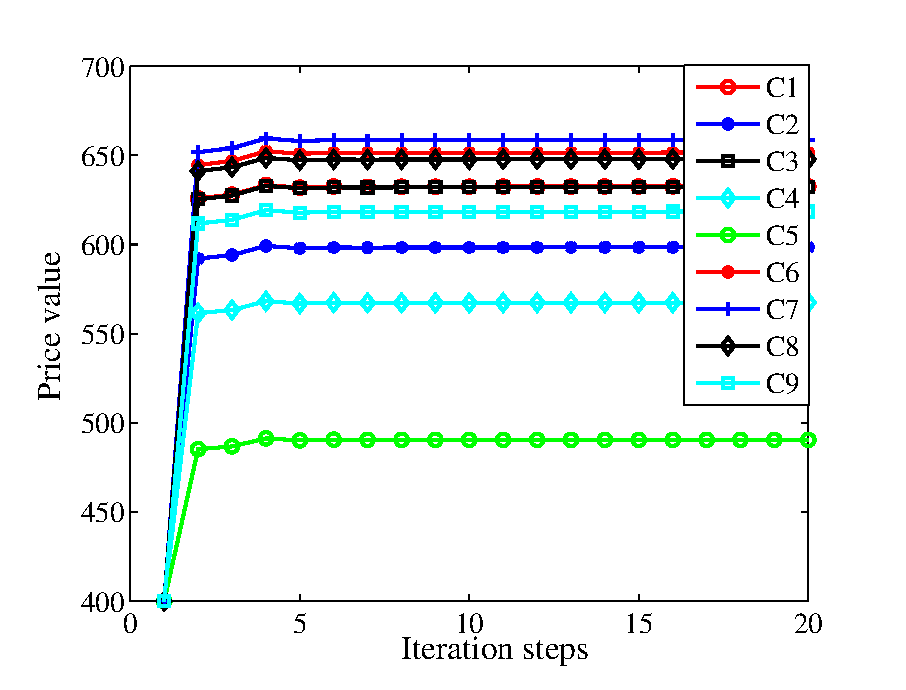
\includegraphics[width=7cm]{3.eps}}
\center{\footnotesize Fig. 3 Price convergence performance.}
\end{figure}

To further verify the performance of the proposed algorithm, Fig. 4 and 5 are completed to verify the robustness and transmission rates of the system. In the heterogenous communication scenarios, serious multi-user interference affects the signal transmission of users, and even causes interruption. As is shown in Fig. 4, the actual outage probabilities of users are always smaller than the given threshold, when $\varepsilon$ varies from 0.1 to 0.4. The results confirmed that not only effective interference management is realized, but also ensures the robust transmission. By comparing with \cite{PCID} and the baseline (The target and actual outage probabilities are equal), all users' actual outage probabilities of this paper are the lowest. This further shows that the proposed algorithm based on robust game is more stable in the practice scenarios with high channel uncertainty.

\begin{figure}[htbp]
\centerline{\includegraphics[width=7cm]{4.eps}}
\center{\footnotesize Fig. 4 Outage probability comparison.}
\end{figure}


As is shown in Fig. 5, the transmission rates of CUE and VUEs in this paper is more balanced than that in \cite{PCID} and \cite{ACAR}. It is because that we have constructed a non-cooperative game framework, where VUEs are selfish and compete for their own profits. In the original problems (11) and (12), the price acts as a key variable to realize the balance among VUEs. When a VUE increases the transmission rate by increasing its power, it will be punished by more interference charges from the BS. Through multiple rounds of game, each user reaches its most satisfactory state, so the transmission rates of users are well balanced and also higher than that in \cite{PCID} and \cite{ACAR}.

\begin{figure}[htbp]
\centerline{\includegraphics[width=7cm]{5.eps}}
\center{\footnotesize Fig. 5 Transmission rate comparison.}
\end{figure}



\section{Conclusion}
In this paper, we have proposed a robust game-based resource allocation algorithm to achieve effective information transmission in the AGHVN. The game relationship between users is focused, real-time power allocation and pricing strategies are formulated to maximize their benefits in the novel optimization scheme. Specifically, to guarantee the system robustness, the probabilistic constraint is introduced to ensure user service reliability and stability. Due to the existence of channel uncertainty, the probability form is non-convex and intractable, the exponential integral method is adopted in the convex optimization process. According to the simulation results, the powers and prices converge to the optimal values in a few steps. We can also conclude that the Stackelberg game optimization scheme shows better robustness. Therefore, the proposed robust game-based resource allocation algorithm is effective under the air-ground integrated heterogeneous vehicular communication scenarios with complex multi-user interference and channel uncertainty.

\begin{thebibliography}{0}
\bibitem{TFL}
W. Lim, J. Huang, Z. Xiong, et al. ``Towards Federated Learning in UAV-Enabled Internet of Vehicles: A Multi-Dimensional ContractMatching Approach," \emph{IEEE Trans. Intelligent Transportation Systems}, vol. 22, no. 8, pp. 5140-5154, Aug. 2021.
\bibitem{ACO}
Q. Wu, J. Xu, Y. Zeng, et al. ``A Comprehensive Overview on 5G-and-Beyond Networks with UAVs: From Communications to Sensing and Intelligence," \emph{IEEE J. Sel. Areas Commun.}, vol. 39, no. 10, pp. 2912-2945, Oct. 2021.
%\bibitem{EMC}
%L. Ruan, J. Wang, J. Chen, et al, ``Energy-Efficient Multi-UAV Coverage Deployment in UAV Networks: A Game-Theoretic Framework, \emph{China Communications}, vol. 15, no. 10, pp.  194-209, Oct. 2018.
\bibitem{ASO}
Y. Xu, G. Gui, H. Gacanin, F. Adachi, ``A survey on resource allocation for 5G heterogeneous networks: Current research, future trends and challenges," \emph{IEEE Commun. Surveys and Tutorials}, vol. 23, no. 2, pp. 668-695, Feb. 2021.
\bibitem{OUC}
H. Wu, F. Lyu, C. Zhou, et al, ``Optimal UAV Caching and Trajectory in Aerial-Assisted Vehicular Networks: A Learning-Based Approach," \emph{IEEE J. Sel. Areas Commun.}, vol. 38, no. 12, pp.  2783-2797, Jun. 2020.
\bibitem{OSI}
N. Kato, Z. Fadlullah, F. Tang, B. Mao, S. Tani, A. Okamura, and J. Liu, ``Optimizing space-air-ground integrated networks by artificial intelligence," \emph{IEEE Wireless Commun.}, vol. 26, no. 4, pp. 140-147, Aug. 2019.
\bibitem{DUE}
M. Liu, J. Yang, and G. Gui, ``Dsf-noma: UAV-assisted emergency communication technology in a heterogeneous internet of things," \emph{IEEE Internet of Things Journal}, vol. 6, no. 3, pp. 5508-5519, Jun. 2019.
\bibitem{SDR}
F. Lyu, P. Yang, H. Wu, et al. ``Service-Oriented Dynamic Resource Slicing and Optimization for Space-Air-Ground Integrated Vehicular Networks," \emph{IEEE Transactions on Intelligent Transportation Systems}, Apr. 2021, DOI:10.1109/TITS.2021.3070542.
\bibitem{HUP}
Q. Han, B. Yang, X. Wang, et al. ``Hierarchical-game-based uplink power control in femtocell networks," \emph{IEEE Trans. Veh. Technol.}, vol. 63, no. 6, pp. 2819-2835, Jul. 2014.
\bibitem{DPC}
K. Zhu, E. Hossain, and A. Anpalagan. ``Downlink Power Control in Two-Tier Cellular OFDMA Networks Under Uncertainties: A Robust Stackelberg Game," \emph{IEEE Trans. commun.}, vol. 63, no. 2, pp. 520-535, Jul. 2015.
\bibitem{CCO}
Z. Liu, Y. Xie, K. Y. Chan, et al. ``Chance-constrained optimization in D2D-based vehicular communication network," \emph{IEEE Trans. Veh. Technol.}, vol. 68, no. 5, pp. 5045-5058, May. 2019.
%\bibitem{TMF}
%D. Zhang, Q. Wu, M. Cui , G. Zhang, and D. Niyato. ``Throughput Maximization for IRS-Assisted Wireless Powered Hybrid NOMA and TDMA," \emph{IEEE Wireless Commun.}, vol. 10, no. 9, pp. 1944-1948, Jun. 2021.
\bibitem{RAI}
Z. Liu, J. Su, Y. Xie, et al. ``Resource Allocation in D2D Enabled Vehicular Communications: A Robust Stackelberg Game Approach Based on Price-Penalty Mechanism," \emph{IEEE Trans. Veh. Technol.}, vol. 70, no. 8, pp. 8186-8200, Jul. 2021.
\bibitem{GT}
G. Owen, ``Game Theory," \emph{New York, NY, USA: Academic}, 2005.
\bibitem{PCID}
Y. Ren, F. Liu, Z. Liu, C. Wang, and Y. Ji, ``Power control in D2D-based vehicular communication networks," \emph{IEEE Trans. Veh. Technol.}, vol. 64, no. 12, pp. 5547-5562, Oct. 2015.
\bibitem{ACAR}
Z. Zhou, Y. Guo, Y. He, et al, ``Access control and resource allocation for M2M communications in industrial automation," \emph{IEEE Trans. Ind. Informat.}, vol. 15, no. 5, pp. 3093-3103, May. 2019.
\end{thebibliography}
\end{document} 